\documentclass[titlepage,12pt]{article}

% Imported Packages
%------------------------------------------------------------------------------
\usepackage{amssymb}
\usepackage{amstext}
\usepackage{amsthm}
\usepackage{amsmath}
\usepackage{enumerate}
\usepackage{fancyhdr}
\usepackage[margin=1in]{geometry}
\usepackage{graphicx}
\usepackage{extarrows}
\usepackage{setspace}

\usepackage{array}
\usepackage{color}
\usepackage[hidelinks]{hyperref}
\usepackage{float}
%------------------------------------------------------------------------------

% Custom commands
%------------------------------------------------------------------------------
\newcounter{myCounter}

%------------------------------------------------------------------------------

% Header and Footer
%------------------------------------------------------------------------------
\pagestyle{plain}
\renewcommand\headrulewidth{0.4pt}
\renewcommand\footrulewidth{0.4pt}
%------------------------------------------------------------------------------

% Title Details
%------------------------------------------------------------------------------
\title{ParkFinder\\Software Requirements Document\\SE 3A04}
\author{Abdul Ahad \\ akhteraa \and Salma Belal \\ belalsm \and Josh Chatten \\ chattejj \and
Nathanael Jordan \\ jordanen \and Robert Stuart \\ stuarr2}
\date{\today}

%------------------------------------------------------------------------------

% Document
%------------------------------------------------------------------------------
\begin{document}

\maketitle	
\thispagestyle{empty}
\clearpage
\setcounter{tocdepth}{2}% Only show down to subsections?
\tableofcontents
\clearpage

\section{Introduction}
\label{sec:introduction}
% Begin Section

%This section should provide an brief overview of the entire document.

\subsection{Purpose}
\label{sub:purpose}
% Begin SubSection

The purpose of this Design Document is to provide a description for the design of the Park Finder
app. The description of the design will allow anyone who will be involved in the development of the
system to proceed with an understanding of what is to be built and how it is expected to be built.
This document provides a description of the system architecture, as well as diagrams that model the
functionality of system, describe the key classes of the system, their interrelationship, and their
responsibilities.

The intended readers of this document include all of the project's stakeholders. This includes the
end-user, the software engineers, and the park authorities.

% End SubSection

\subsection{System Description}
\label{sub:system_description}
%Begin SubSection

The software system being described in this document is called the ParkFinder app. This system will
have datasets of information about parks from all over the world and will allow the client to use
search methods in order to find parks based on the clients' desired attributes. The app is meant to
be used anywhere in the world, provided an Android or iOS device with the app installed. This
provides clients with an easier, faster, and more efficient way to look up parks and acquire
information such as the location, facilities, activities, and rentals that the parks provide.

% End SubSection

\subsection{Overview}
\label{sub:overview}
% Begin SubSection

The remainder of this document will contain diagrams and information that will describe the details
for the software system being built. This will include a use case diagram in Section~
\ref{sec:use_case_diagram}, an analysis class diagram in Section~\ref{sec:analysis_class_diagram}, a
description of the architectural design in Section~\ref{sec:architectural_design}, and CRC cards for
all identified classes in Section~\ref{sec:class_responsibility_collaboration_crc_cards}.

% End SubSection

% End Section

\section{Use Case Diagram}
\label{sec:use_case_diagram}
% Begin Section

\begin{figure}[htbp]
\centerline{\includegraphics[width=0.99\textwidth]{images//UseCase}}
\caption{Use Case Diagram}
\label{useCaseDiagram}
\end{figure}

\begin{enumerate}[a)]
    \item \textbf{Search for parks:} The user searches for parks. This is accomplished by consulting
    experts based on which park attributes were selected by the user.
    \item \textbf{Browse park's listing} User browses a list of parks, this list can either be the
    result of a previous search action or a default list (all parks).
    \item \textbf{Select park(s):} User selects a park or several parks from the list they were
    browsing, this displays additional park information to the user as well as the park(s) on a map
    if desired.
    \item \textbf{Request nearest 5 parks:} User requests the five nearest parks to their current
    location.
    \item \textbf{Swap or remove expert:} A developer attempts to swap or remove an expert from the
    system, the system requires authorization from a manager for the change to occur.
\end{enumerate}

% End Section

\section{Analysis Class Diagram}
\label{sec:analysis_class_diagram}
% Begin Section

\begin{figure}[H]
	\centerline{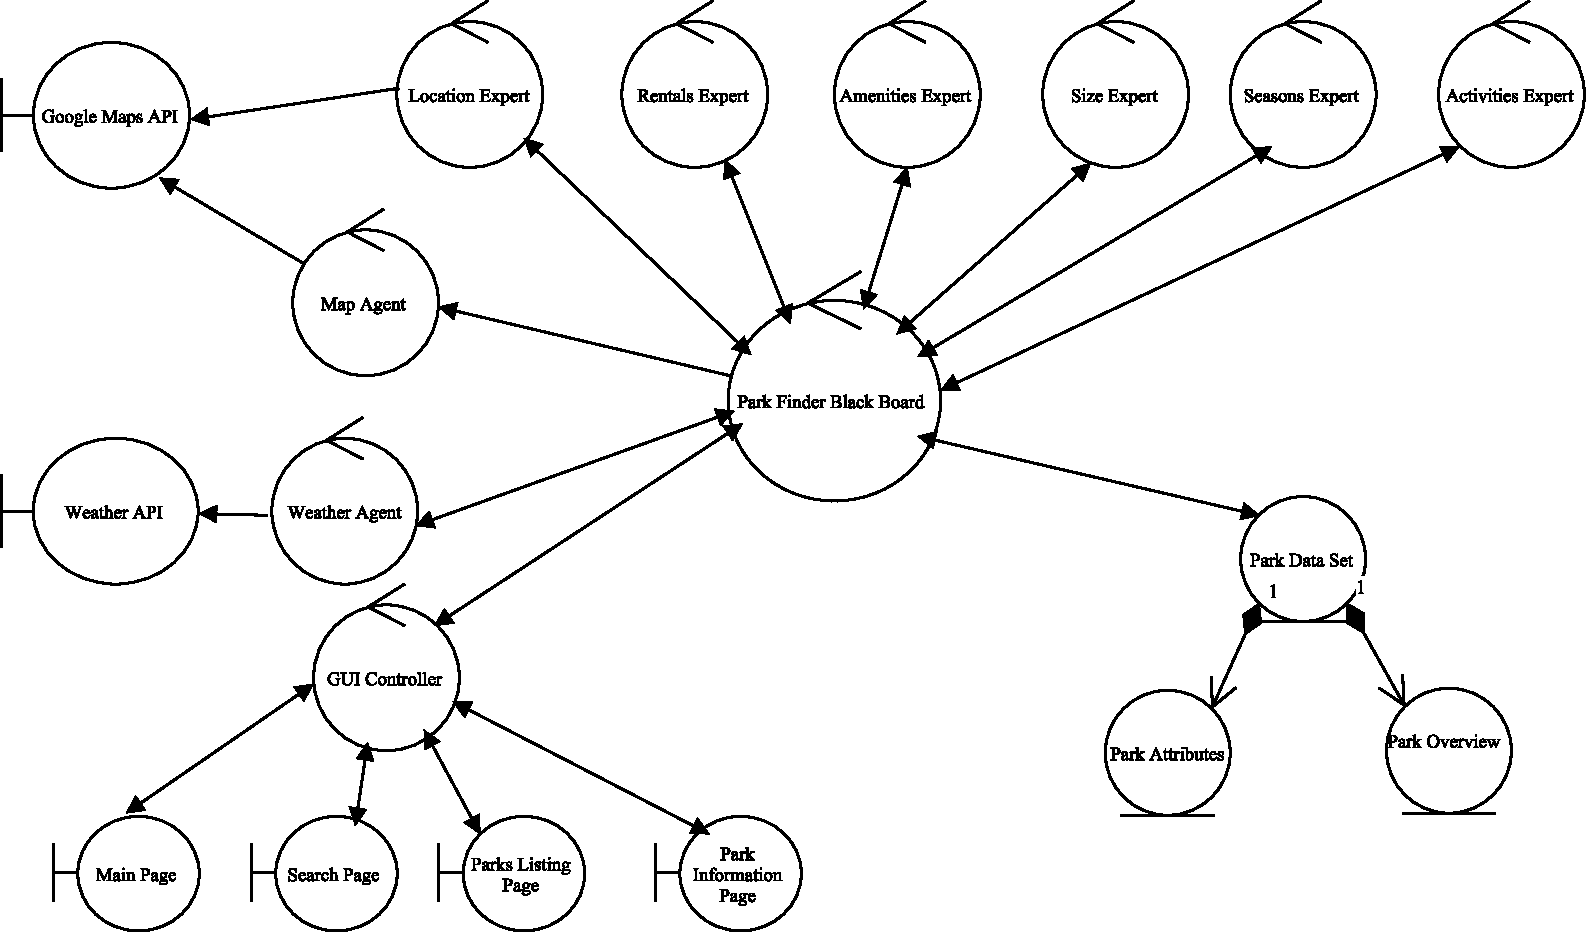
\includegraphics[width=0.99\textwidth]{images//analysis_class_diagram}}
	\caption{Analysis Class Diagram}
	\label{analysisClassDiagram}
\end{figure}

% End Section

\section{Architectural Design}
\label{sec:architectural_design}
% Begin Section

%This section should provide an overview of the overall architectural design of your application.
%Your overall architecture should show the division of the system into subsystems with high
%cohesion and low coupling.

\subsection{System Architecture}
\label{sub:system_architecture}
% Begin SubSection

%\begin{enumerate}[a)]
%    \item Identify and explain the overall architecture of your system
%    \item Be sure to clearly state the name of the architecture
%    \item Provide the reasoning and justification of the choice
%    \item Provide a structural architecture diagram showing the relationship among the subsystems
%    (if appropriate)
%\end{enumerate}
The application uses a blackboard architecture which incorporates eight independent subsystems that all interact with the blackboard, the ParkFinder application. These independent subsystems are the Location Expert, Rentals Expert, Amenities Expert, Size Expert, Seasons Expert, Activities Expert, Map Agent and Weather Agent. The blackboard includes a data store for parks and also interacts with a controller.\newline 

\begin{figure}[H]
	\centerline{\includegraphics[width=0.99\textwidth]{images//architecture}}
	\caption{Structural Architecture Diagram}
	\label{useCaseDiagram}
\end{figure} 

By using the blackboard architecture style, as seen above in Figure 3, a modularized and intuitive design is achieved by having independence between knowledge sources. This independence implies high cohesion and low coupling, allowing changes or updates to the knowledge sources with ease. 


% End SubSection

\subsection{Subsystems}
\label{sub:subsystems}
% Begin SubSection

The system will be divided into several different subsystems that are shown in Figure~
\ref{analysisClassDiagram}. Each of these subsystems will handle different functionality of the
overall system. The GUI and User subsystems will handle all interactions with the user of the
application. The database will contain all of the information about each park in the system. The
several Expert subsystems will have similar functionality but handle different information. Each
Expert subsystem will be provided search criteria and will return all parks which satisfy the
criteria. The Weather Agent will provide the weather at any requested location. Lastly, ParkFinder
will handle the information flow between all of the subsystems. ParkFinder will receive the user
search criteria from GUI then provide that information and the database to the appropriate Expert(s)
in order to identify the correct park.

% End SubSection

% End Section
    
\section{Class Responsibility Collaboration (CRC) Cards}
\label{sec:class_responsibility_collaboration_crc_cards}
% Begin Section

%This section should contain all of your CRC cards.
%

    \begin{table}[H]
        \centering
        \begin{tabular}{|p{5cm}|p{5cm}|}
        \hline 
        \multicolumn{2}{|l|}{\textbf{Class Name: Main Page}} \\
        \hline
        \textbf{Responsibility:} & \textbf{Collaborators:} \\
        \hline
        Handles click events of "Start Search" Button & GUI Controller\\
        \hline
        Handles click events of “View All Parks” button	&	GUI Controller\\
        \hline
        Handles click events of “Find Nearest 5 Parks” button & GUI Controller
\\
\hline        \end{tabular}
    \end{table}
    
    
 \begin{table}[H]
 	\centering
 	\begin{tabular}{|p{5cm}|p{5cm}|}
 		\hline 
 		\multicolumn{2}{|l|}{\textbf{Class Name: Search Page}} \\
 		\hline
 		\textbf{Responsibility:} & \textbf{Collaborators:} \\
 		\hline
	 	Knows Search Criteria & \\ 
	 	\hline
	 	Knows GUI Controller &\\
 		\hline
 		Handles click events of selecting a search criterion	&	GUI Controller\\
 		\hline
 		Handles click events of the "Search" Button		&	GUI Controller\\
 		\hline
 		Handles click events of the "Back to main page" Button	&	GUI Controller\\
 		\hline        \end{tabular}
 \end{table}
 	\begin{table}[H]
 		\centering
 		\begin{tabular}{|p{5cm}|p{5cm}|}
 			\hline 
 			\multicolumn{2}{|l|}{\textbf{Class Name:Park Listings Page}} \\
 			\hline
 			\textbf{Responsibility:} & \textbf{Collaborators:} \\
 			\hline
 			Knows GUI Controller & \\
 			\hline
 			Displays park names that are a result of the selected search criteria, or all available parks	&		GUI Controller\\
 			\hline
 			Handles click events for selecting a park 			&	GUI Controller\\
 			\hline
 			Handles click events of the “view the listed parks on a map” Button	& GUI Controller\\
 			\hline
 			Handles click events of the “Back to search page” button		& GUI Controller\\
 			\hline
 			
 		\end{tabular}
 		
 		
 		
 	\end{table}
 	
 		\begin{table}[H]
 			\centering
 			\begin{tabular}{|p{5cm}|p{5cm}|}
 				\hline 
 				\multicolumn{2}{|l|}{\textbf{Class Name:Park Information Page}} \\
 				\hline
 				\textbf{Responsibility:} & \textbf{Collaborators:} \\
 				\hline
 				Knows park name		&	GUI Controller\\
 				\hline
 				Displays park overview			& GUI Controller	\\
 				\hline
 				Displays park attributes		& GUI Controller \\
 				\hline
 				Handles click events for the “back to park listings page” button	&	GUI Controller\\
 				\hline
 			\end{tabular}
 		\end{table}
 		
 		\begin{table}[H]
 			\centering
 			\begin{tabular}{|p{5cm}|p{5cm}|}
 				\hline 
 				\multicolumn{2}{|l|}{\textbf{Class Name:GUI Controller}} \\
 				\hline
 				\textbf{Responsibility:} & \textbf{Collaborators:} \\
 				\hline
 				Knows Search Page & \\
 				\hline
 				Knows Main Page & \\
 				\hline
 				Knows Park Listings Page &\\
 				\hline
				Knows Park Information Page &\\
				\hline
				Knows Park Finder Black Board &\\
				\hline
				Controls which pages are displayed to the user and when to switch from one page to another page	&	Search Page, Main Page, Park Listings Page, Park Information Page\\
				\hline
				Controls the parks being displayed in the park listings page &	Park Listings Page, Park Finder Black Board \\
				\hline
				Controls the park information being displayed in the park &	Park Information Page, Park Information Page Finder Black Board 	\\
				\hline
				Gives the user’s desired search criterion to the system &	Search Page, Park Finder Black Board\\
				
 				\hline
 			\end{tabular}
 		\end{table}
 		
 		 			\begin{table}[H]
 		 				\centering
 		 				\begin{tabular}{|p{5cm}|p{5cm}|}
 		 					\hline 
 		 					\multicolumn{2}{|l|}{\textbf{Class Name:Park Data Set}} \\
 		 					\hline
 		 					\textbf{Responsibility:} & \textbf{Collaborators:} \\
 		 					\hline
	 		 				 Knows Park  & \\
	 		 				 \hline
	 		 				 Knows Park Attributes & \\
	 		 				 \hline
	 		 				 Knows Park Overview&\\
	 		 				 \hline
	 		 				 Knows Park Finder Black Board&\\
	 		 				 \hline
	 		 				 Owns Park Attributes	& Park Attributes\\
	 		 				 \hline
	 		 				 Owns Park Overview	& Park Overview\\
	 		 				 \hline
	 		 				 Allows Park Finder Black Board to read park data 	& Park Finder Black Board \\
 		 					\hline
 		 				\end{tabular}
 		 			\end{table}
 		
 				\begin{table}[H]
 					\centering
 					\begin{tabular}{|p{5cm}|p{5cm}|}
 						\hline 
 						\multicolumn{2}{|l|}{\textbf{Class Name: Park Overview}} \\
 						\hline
 						\textbf{Responsibility:} & \textbf{Collaborators:} \\
 						\hline
 					    Knows Park Data Set (Owner)& \\
 					    \hline
 					    Knows Park & \\
 					    \hline
 					    Knows Park’s Overview (highlights of the
 					    park, the address, phone number, website, and operational
 					    dates) & \\
 					    \hline
 						Each park overview belongs to the owner park	& Park Data Set\\
 						\hline
 						
 						
 					\end{tabular}
 				\end{table}
 		
 		\begin{table}[H]
 			\centering
 			\begin{tabular}{|p{5cm}|p{5cm}|}
 				\hline 
 				\multicolumn{2}{|l|}{\textbf{Class Name:Park Attributes}} \\
 				\hline
 				\textbf{Responsibility:} & \textbf{Collaborators:} \\
 				\hline
 				Knows Park Data Set (Owner) & \\
 				\hline
 				Knows Park & \\
 				\hline
 				Knows Park’s attributes (amenities, size, seasons open, 
 				activities, and rentals) & \\
 				\hline
 				Each set of park attributes belongs to the owner park &	Park Data Set\\
 				
 				\hline
 				
 			\end{tabular}
 		\end{table}
 		
 		
 				\begin{table}[H]
 					\centering
 					\begin{tabular}{|p{5cm}|p{5cm}|}
 						\hline 
 						\multicolumn{2}{|l|}{\textbf{Class Name:Activities Expert}} \\
 						\hline
 						\textbf{Responsibility:} & \textbf{Collaborators:} \\
 						\hline
 						Knows Activities & \\
 						\hline
 						Knows Park Finder Black Board & \\
 						\hline
 						Uses knowledge of activities to find parks with specified activities &	Park Finder Black Board \\
 						\hline
 					\end{tabular}
 				\end{table}
 		
 				\begin{table}[H]
 					\centering
 					\begin{tabular}{|p{5cm}|p{5cm}|}
 						\hline 
 						\multicolumn{2}{|l|}{\textbf{Class Name:Amenities Expert}} \\
 						\hline
 						\textbf{Responsibility:} & \textbf{Collaborators:} \\
 						\hline
 						Knows Amenities & \\
 						\hline
 						Knows Park Finder Black Board & \\
 						\hline
 						Uses knowledge of amenities to find parks with specified amenities  &	Park Finder Black Board \\
 						\hline
 					\end{tabular}
 				\end{table}	
 				
 				
 				\begin{table}[H]
 					\centering
 					\begin{tabular}{|p{5cm}|p{5cm}|}
 						\hline 
 						\multicolumn{2}{|l|}{\textbf{Class Name:Rentals Expert}} \\
 						\hline
 						\textbf{Responsibility:} & \textbf{Collaborators:} \\
 						\hline
 						Knows Rentals & \\
 						\hline
 						Knows Park Finder Black Board & \\
 						\hline
 						Uses knowledge of rentals to find parks with specified rentals &	Park Finder Black Board \\
 						\hline
 					\end{tabular}
 				\end{table}	
 				
 				\begin{table}[H]
 					\centering
 					\begin{tabular}{|p{5cm}|p{5cm}|}
 						\hline 
 						\multicolumn{2}{|l|}{\textbf{Class Name:Size Expert}} \\
 						\hline
 						\textbf{Responsibility:} & \textbf{Collaborators:} \\
 						\hline
 						Knows Sizes & \\
 						\hline
 						Knows Park Finder Black Board & \\
 						\hline
 						Uses knowledge of sizes to find parks with specified size &	Park Finder Black Board \\
 						\hline
 					\end{tabular}
 				\end{table}	
 				
 				\begin{table}[H]
 					\centering
 					\begin{tabular}{|p{5cm}|p{5cm}|}
 						\hline 
 						\multicolumn{2}{|l|}{\textbf{Class Name:Location Expert}} \\
 						\hline
 						\textbf{Responsibility:} & \textbf{Collaborators:} \\
 						\hline
 						Knows Google Maps API & \\
 						\hline
 						Knows Locations & \\
 						\hline
 						Knows Park Finder Black Board & \\
 						\hline
 						Uses knowledge of locations to find nearest 5 parks &	Park Finder Black Board, Google Maps API \\
 						\hline
 					\end{tabular}
 				\end{table}	
 				
 				\begin{table}[H]
 					\centering
 					\begin{tabular}{|p{5cm}|p{5cm}|}
 						\hline 
 						\multicolumn{2}{|l|}{\textbf{Class Name:Seasons Expert}} \\
 						\hline
 						\textbf{Responsibility:} & \textbf{Collaborators:} \\
 						\hline
 						Knows Seasons & \\
 						\hline
 						Knows Park Finder Black Board & \\
 						\hline
 						Uses knowledge of Seasons to find parks with specified operating season & Park Finder Black Board \\
 						\hline
 					\end{tabular}
 				\end{table}	
 				
 				\begin{table}[H]
 					\centering
 					\begin{tabular}{|p{5cm}|p{5cm}|}
 						\hline 
 						\multicolumn{2}{|l|}{\textbf{Class Name:Weather Agent}} \\
 						\hline
 						\textbf{Responsibility:} & \textbf{Collaborators:} \\
 						\hline
 						Knows Park Location & \\
 						\hline
 						Knows Weather API & \\
 						\hline
 						Knows Park Finder Black Board & \\
 						\hline
 						Uses knowledge of Park Location to get weather at that location  &	Park Finder Black Board, Weather API \\
 						\hline
 					\end{tabular}
 				\end{table}	
 				\begin{table}[H]
 					\centering
 					\begin{tabular}{|p{5cm}|p{5cm}|}
 						\hline 
 						\multicolumn{2}{|l|}{\textbf{Class Name: 						Park Finder Black Board}} \\
 						\hline
 						\textbf{Responsibility:} & \textbf{Collaborators:} \\
 						\hline

 						Knows Weather Agent & \\ \hline
 						Knows Google Maps API & \\ \hline
 						Knows GUI Controller & \\ \hline
 						Knows Park Data Set & \\ \hline
 						Knows Location Expert & \\ \hline
 						Knows Rentals Expert & \\ \hline
 						Knows Amenities Expert & \\ \hline
 						Knows Size Expert & \\ \hline
 						Knows Seasons Expert & \\ \hline
 						Knows Activities Expert  & \\ \hline
 						Knows the search criterion that the user requested and &	All Experts, Search Page
 						tells each expert its relevant search criteria\\ \hline
 						Knows the results of all search requests & 	All Experts, Park Data Set\\ \hline
 						Sends search results and park information to the GUI	& GUI Controller, Park Data set\\ \hline
 						Accesses the weather agent and sends the retrieved information to the GUI	& Weather Agent, GUI Controller\\ \hline
 						Sends park locations to the Map Agent	& Map Agent, Park Data Set\\ \hline
 					\end{tabular}
 				\end{table}		
 			
 				\begin{table}[H]
 					\centering
 					\begin{tabular}{|p{5cm}|p{5cm}|}
 						\hline 
 						\multicolumn{2}{|l|}{\textbf{Class Name:Map Agent}} \\
 						\hline
 						\textbf{Responsibility:} & \textbf{Collaborators:} \\
 						\hline
 						Knows Park Location & \\
 						\hline
 						Knows Google Maps API & \\
 						\hline
 						Knows Park Finder Black Board & \\
 						\hline
 				Sends locations to the Google Maps API to display Parks On the Map  &	Park Finder Black Board, Google Maps API API \\
 						\hline
 					\end{tabular}
 				\end{table}		
 
 				
% End Section

\newpage
\appendix
\section{Division of Labour}%TODO
\label{sec:division_of_labour}
% Begin Section

\begin{table}[H]
\vspace{-0.06in}
\begin{center}
\setlength{\extrarowheight}{4.0pt}
\begin{tabular}{m{0.3\textwidth} m{0.2\textwidth} m{0.3\textwidth}} 
\hline
\textbf{Contributions} & \textbf{Name} & \textbf{Signature}\\
\hline
x & Abdul Ahad & \\
\hline
x & Salma Belal & \\
\hline
x & Josh Chatten & \\
\hline
x & Nathanael Jordan  & \\
\hline
x & Robert Stuart & \\
\hline
\end{tabular}
\end{center}
\label{divOfLabour}
\end{table}

% End Section

%\newpage
%\section*{IMPORTANT NOTES}
%\begin{itemize}
%%   \item You do \underline{NOT} need to provide a text explanation of each diagram; the diagram
%% should speak for itself
%    \item Please document any non-standard notations that you may have used
%    \begin{itemize}
%        \item \emph{Rule of Thumb}: if you feel there is any doubt surrounding the meaning of your
%        notations, document them
%    \end{itemize}
%    \item Some diagrams may be difficult to fit into one page
%    \begin{itemize}
%        \item It is OK if the text is small but please ensure that it is readable when printed
%        \item If you need to break a diagram onto multiple pages, please adopt a system of doing so
%        and thoroughly explain how it can be reconnected from one page to the next; if you are
%        unsure about this, please ask about it
%    \end{itemize}
%    \item Please submit the latest version of Deliverable 1 with Deliverable 2
%    \begin{itemize}
%        \item It does not have to be a freshly printed version; the latest marked version is OK
%    \end{itemize}
%    \item If you do \underline{NOT} have a Division of Labour sheet, your deliverable will
%    \underline{NOT} be marked
%\end{itemize}

\end{document}
%------------------------------------------------------------------------------